% ============================================================
%  J3 — APRÈS-MIDI : PyTorch & CNN
%  Julien Rolland — M2 Développement Fullstack
% ============================================================
\documentclass[aspectratio=169, 10pt]{beamer}
% ============================================================
%  PREAMBLE COMMUN — IA, Deep Learning & Machine Learning
%  Julien Rolland — M2 Développement Fullstack
% ============================================================

% --- Langue & encodage ---
\usepackage[utf8]{inputenc}
\usepackage[T1]{fontenc}
\usepackage{babel}
\babelprovide[import, main]{french}

% --- Thème Beamer ---
\usetheme{Madrid}
\usecolortheme{default}

% Palette de bleu académique
\definecolor{jedy_blue}{RGB}{0, 51, 102}       % bleu foncé principal
\definecolor{jedy_mid}{RGB}{0, 102, 179}        % bleu moyen accent
\definecolor{jedy_light}{RGB}{204, 221, 240}    % bleu très clair (fond boxes)
\definecolor{jedy_alert}{RGB}{180, 30, 30}      % rouge pour alertes
\definecolor{jedy_example}{RGB}{0, 120, 60}     % vert pour exemples

% Application des couleurs sur le thème Madrid
\setbeamercolor{palette primary}{bg=jedy_blue, fg=white}
\setbeamercolor{palette secondary}{bg=jedy_mid, fg=white}
\setbeamercolor{palette tertiary}{bg=jedy_blue, fg=white}
\setbeamercolor{palette quaternary}{bg=jedy_blue, fg=white}
\setbeamercolor{structure}{fg=jedy_blue}
\setbeamercolor{frametitle}{bg=jedy_blue, fg=white}
\setbeamercolor{title}{bg=jedy_blue, fg=white}
\setbeamercolor{block title}{bg=jedy_mid, fg=white}
\setbeamercolor{block body}{bg=jedy_light, fg=black}
\setbeamercolor{block title alerted}{bg=jedy_alert, fg=white}
\setbeamercolor{block body alerted}{bg=jedy_light, fg=black}
\setbeamercolor{block title example}{bg=jedy_example, fg=white}
\setbeamercolor{block body example}{bg=jedy_light, fg=black}

% --- Typographie ---
\usepackage{lmodern}
\setbeamerfont{title}{size=\Large, series=\bfseries}
\setbeamerfont{frametitle}{size=\normalsize, series=\bfseries}

% --- Navigation : suppression des icônes de navigation par défaut ---
\setbeamertemplate{navigation symbols}{}

% --- Numérotation des slides ---
\setbeamertemplate{footline}{%
  \leavevmode%
  \hbox{%
    \begin{beamercolorbox}[wd=.333\paperwidth,ht=2.25ex,dp=1ex,center]{author in head/foot}%
      \usebeamerfont{author in head/foot}\insertshortauthor
    \end{beamercolorbox}%
    \begin{beamercolorbox}[wd=.334\paperwidth,ht=2.25ex,dp=1ex,center]{title in head/foot}%
      \usebeamerfont{title in head/foot}\insertshorttitle
    \end{beamercolorbox}%
    \begin{beamercolorbox}[wd=.333\paperwidth,ht=2.25ex,dp=1ex,right]{date in head/foot}%
      \usebeamerfont{date in head/foot}
      \insertframenumber{} / \inserttotalframenumber\hspace*{2ex}
    \end{beamercolorbox}%
  }%
  \vskip0pt%
}

% --- Maths ---
\usepackage{amsmath, amssymb, amsthm}
\usepackage{bm}          % vecteurs en gras : \bm{w}

% --- Code source ---
\usepackage{listings}
\usepackage{xcolor}

\lstdefinestyle{pythonstyle}{
  language=Python,
  basicstyle=\ttfamily\footnotesize,
  keywordstyle=\color{jedy_blue}\bfseries,
  commentstyle=\color{gray}\itshape,
  stringstyle=\color{jedy_example},
  numberstyle=\tiny\color{gray},
  numbers=left,
  numbersep=5pt,
  frame=single,
  framerule=0.4pt,
  rulecolor=\color{jedy_light},
  backgroundcolor=\color{jedy_light!40},
  breaklines=true,
  showstringspaces=false,
  tabsize=4,
}
\lstset{style=pythonstyle}

% Alias pratique pour code inline
\newcommand{\code}[1]{\texttt{\small#1}}

% --- Graphiques ---
\usepackage{graphicx}
\usepackage{tikz}
\usetikzlibrary{arrows.meta, positioning, shapes.geometric, fit, calc}
\usepackage{pgfplots}
\pgfplotsset{compat=1.18}

% --- Tableaux ---
\usepackage{booktabs}
\usepackage{array}

% --- Icônes (optionnel, nécessite fontawesome5) ---
% \usepackage{fontawesome5}

% --- Macros ML/DL courantes ---
\newcommand{\R}{\mathbb{R}}
\newcommand{\E}{\mathbb{E}}
\newcommand{\Loss}{\mathcal{L}}
\newcommand{\dataset}{\mathcal{D}}
\newcommand{\X}{\mathbf{X}}
\newcommand{\y}{\mathbf{y}}
\newcommand{\w}{\mathbf{w}}
\newcommand{\W}{\mathbf{W}}
\newcommand{\grad}{\nabla}
\newcommand{\T}{^{\top}}         % transposée : \X\T
\newcommand{\lr}{\alpha}         % learning rate
\newcommand{\norm}[1]{\left\|#1\right\|}

% Encadré "Objectif pédagogique" en début de section
\newenvironment{objectif}{%
  \begin{alertblock}{Objectif}%
}{%
  \end{alertblock}%
}

% --- Infos du cours (remplacer dans chaque slides.tex) ---
\author[J. Rolland]{Julien Rolland}
\institute[Jedy]{Formation M2 Développement Fullstack}


\title[PyTorch \& CNN]{PyTorch \& Réseaux de Neurones Convolutifs}
\subtitle{Jour 3 --- Après-midi}
\date{Jour 3}

% ============================================================
\begin{document}
% ============================================================

\begin{frame}
  \titlepage
\end{frame}

\begin{frame}{Plan du module}
  \tableofcontents
\end{frame}

% ============================================================
\section{Vers PyTorch}
% ============================================================

\begin{frame}{Pourquoi passer à PyTorch ?}
  \begin{columns}[T]
    \begin{column}{0.48\textwidth}
      \begin{alertblock}{Limite du «~fait main~» (J3-AM)}
        \begin{itemize}
          \item Notre classe \code{Value} est \textbf{pédagogique} mais lente
          \item Python pur : quelques milliers d'opérations/s
          \item Un vrai réseau : \textbf{milliards} d'opérations par forward
        \end{itemize}
      \end{alertblock}
      \smallskip
      \begin{exampleblock}{Même principe, autre échelle}
        Même graphe de calcul, même \code{backward()}\\
        $\Rightarrow$ mais sur des \textbf{tenseurs} en C++/CUDA
      \end{exampleblock}
    \end{column}
    \begin{column}{0.48\textwidth}
      \begin{block}{La solution industrielle}
        \begin{itemize}
          \item \textbf{Calcul vectorisé} : matrices entières en une opération
          \item \textbf{Backend C++/CUDA} : parallélisme GPU
          \item \textbf{Écosystème riche} :
            \begin{itemize}
              \item \code{torchvision} — Vision par ordinateur
              \item \code{torchaudio} — Audio
              \item \code{transformers} — NLP / LLM
            \end{itemize}
        \end{itemize}
      \end{block}
    \end{column}
  \end{columns}
\end{frame}

% ============================================================
\section{Tenseurs}
% ============================================================

\begin{frame}{Le Concept de Tenseur (\texttt{torch.Tensor})}
  \begin{columns}[T]
    \begin{column}{0.44\textwidth}
      \begin{block}{Définition}
        Généralisation des matrices à $n$ dimensions\\[0.3em]
        \begin{center}
          scalaire $\subset$ vecteur $\subset$ matrice $\subset$ tenseur
        \end{center}
      \end{block}
      \smallskip
      \begin{block}{Propriétés clés}
        \begin{itemize}
          \item \code{shape} : géométrie du tenseur
          \item \code{device} : CPU ou GPU (\code{cuda})
          \item \code{grad} : stockage du gradient \\
                {\small $\Rightarrow$ notre \code{self.grad} de ce matin}
          \item \code{requires\_grad} : active l'autograd
        \end{itemize}
      \end{block}
    \end{column}
    \begin{column}{0.52\textwidth}
      \begin{center}
        \renewcommand{\arraystretch}{1.4}
        \begin{tabular}{lll}
          \toprule
          \textbf{Objet} & \textbf{Shape} & \textbf{Cas d'usage} \\
          \midrule
          Scalaire  & \code{[]}           & Perte $\Loss$ \\
          Vecteur   & \code{[n]}          & Biais, sortie \\
          Matrice   & \code{[n, m]}       & Poids $\W$ \\
          Batch     & \code{[B, n]}       & Mini-batch \\
          Image     & \code{[B, C, H, W]} & Batch d'images \\
          \bottomrule
        \end{tabular}
      \end{center}
      \smallskip
      \begin{exampleblock}{Exemple : batch d'images RGB}
        \code{[128, 3, 224, 224]}\\
        {\small 128 images $\cdot$ 3 canaux $\cdot$ $224\times224$ pixels}
      \end{exampleblock}
    \end{column}
  \end{columns}
\end{frame}

% ============================================================
\section{torch.nn}
% ============================================================

\begin{frame}[fragile]{La Philosophie \texttt{torch.nn}}
  \begin{columns}[T]
    \begin{column}{0.38\textwidth}
      \begin{block}{Le \texttt{Module} : brique de base}
        \begin{itemize}\small
          \item On ne gère \textbf{plus} $\W$ et $\bm{b}$ manuellement
          \item \code{nn.Linear}, \code{nn.Conv2d}... gèrent leurs paramètres
          \item \code{\_\_init\_\_} : définit les couches
          \item \code{forward()} : flux de données
        \end{itemize}
      \end{block}
      \smallskip
      \begin{exampleblock}{Avantage}
        \small\code{model.parameters()} retourne\\
        \textbf{tous} les poids $\Rightarrow$ prêts pour l'optimiseur
      \end{exampleblock}
    \end{column}
    \begin{column}{0.58\textwidth}
      \begin{lstlisting}[style=pythonstyle]
import torch.nn as nn
import torch.nn.functional as F

class MLP(nn.Module):
    def __init__(self, n_in, n_h, n_out):
        super().__init__()
        self.fc1 = nn.Linear(n_in, n_h)
        self.fc2 = nn.Linear(n_h, n_out)

    def forward(self, x):
        x = F.relu(self.fc1(x))
        return self.fc2(x)

model = MLP(784, 128, 10)
# Nombre de parametres :
n = sum(p.numel() for p in model.parameters())
print(f"{n} parametres")  # 101770
      \end{lstlisting}
    \end{column}
  \end{columns}
\end{frame}

% ============================================================
\section{Optimisation \& Data}
% ============================================================

\begin{frame}[fragile]{Optimisation et Data Handling}
  \begin{columns}[T]
    \begin{column}{0.44\textwidth}
      \begin{block}{\texttt{torch.optim} : plus de \code{w -= lr*grad}}
        \begin{itemize}\small
          \item \textbf{SGD} : descente de gradient classique
          \item \textbf{Adam} : adaptatif, converge rapidement
          \item \textbf{RMSprop} : stable pour les RNN
        \end{itemize}
      \end{block}
      \smallskip
      \begin{block}{\texttt{Dataset} \& \texttt{DataLoader}}
        \begin{itemize}\small
          \item \code{Dataset} : comment accéder à un exemple
          \item \code{DataLoader} : gère le \textbf{batching},\\
                le \textbf{shuffling} et le \textbf{multi-threading}
          \item Le GPU ne doit pas attendre le CPU
        \end{itemize}
      \end{block}
    \end{column}
    \begin{column}{0.52\textwidth}
      \begin{lstlisting}[style=pythonstyle]
import torch.optim as optim
from torch.utils.data import DataLoader

# Optimiseur Adam
opt = optim.Adam(model.parameters(), lr=1e-3)

# DataLoader
loader = DataLoader(
    dataset,
    batch_size=32,
    shuffle=True,
    num_workers=4,   # threads CPU
)

for X, y in loader:
    # X.shape = [32, ...]
    pass
      \end{lstlisting}
    \end{column}
  \end{columns}
\end{frame}

% ============================================================
\section{Convolutions}
% ============================================================

\begin{frame}{Pourquoi le MLP Échoue sur les Images ?}
  \begin{columns}[T]
    \begin{column}{0.48\textwidth}
      \begin{alertblock}{Problème 1 : Explosion des paramètres}
        \begin{itemize}
          \item Image $1024 \times 1024 \Rightarrow 10^6$ entrées
          \item Couche cachée de 512 neurones
          \item $10^6 \times 512 = \mathbf{5 \times 10^8}$ poids
          \item Rien que pour la \textbf{première couche} !
        \end{itemize}
      \end{alertblock}
      \smallskip
      \begin{alertblock}{Problème 2 : Perte de topologie}
        \begin{itemize}
          \item Flatten $\Rightarrow$ perte de la \textbf{structure 2D}
          \item Un décalage d'1 pixel change tout le vecteur
          \item Le réseau ne voit pas la \textbf{proximité spatiale}
        \end{itemize}
      \end{alertblock}
    \end{column}
    \begin{column}{0.48\textwidth}
      \begin{exampleblock}{Solution : CNN}
        \begin{itemize}
          \item \textbf{Localité} : chaque neurone voit une petite zone
          \item \textbf{Partage des poids} : même filtre sur toute l'image
          \item \textbf{Hiérarchie} : bords $\to$ formes $\to$ objets
        \end{itemize}
      \end{exampleblock}
      \smallskip
      \begin{center}
        \renewcommand{\arraystretch}{1.3}
        \begin{tabular}{lrr}
          \toprule
           & \textbf{MLP} & \textbf{CNN} \\
          \midrule
          Params ($1^{\text{re}}$ couche) & $500\text{M}$ & $\sim 1\text{K}$ \\
          Invariance translation & Non & Oui \\
          Localité spatiale & Non & Oui \\
          \bottomrule
        \end{tabular}
      \end{center}
    \end{column}
  \end{columns}
\end{frame}

\begin{frame}{La Convolution : Extraction de Features}
  \begin{columns}[T]
    \begin{column}{0.44\textwidth}
      \begin{block}{Le Kernel (Filtre)}
        \begin{itemize}
          \item Petite fenêtre (ex: $3 \times 3$) qui \textbf{glisse} sur l'image
          \item \textbf{Localité} : chaque neurone ne voit qu'une zone
          \item \textbf{Partage des poids} : même filtre partout
          \item $\Rightarrow$ beaucoup moins de paramètres
        \end{itemize}
      \end{block}
      \smallskip
      \begin{exampleblock}{Ce que le réseau apprend}
        Couche 1 : bords, contrastes\\
        Couche 2 : coins, textures\\
        Couche $n$ : visages, objets\ldots
      \end{exampleblock}
    \end{column}
    \begin{column}{0.52\textwidth}
      \centering
      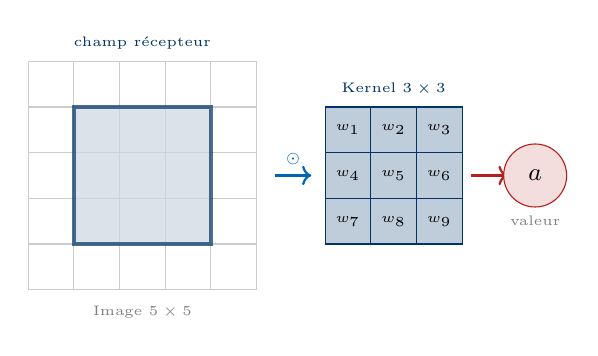
\begin{tikzpicture}[scale=0.58]
        % --- Input 5x5 ---
        \foreach \i in {0,...,4} {
          \foreach \j in {0,...,4} {
            \draw[gray!40] (\i,\j) rectangle ++(1,1);
          }
        }
        % Highlighted receptive field 3x3 at (1,1)
        \draw[jedy_blue, very thick, fill=jedy_blue!20, opacity=0.7]
          (1,1) rectangle ++(3,3);
        \node[font=\tiny, gray] at (2.5, -0.5) {Image $5 \times 5$};
        \node[font=\tiny, color=jedy_blue] at (2.5, 5.4) {champ récepteur};

        % --- Arrow ---
        \draw[->, thick, jedy_mid] (5.4, 2.5) -- (6.2, 2.5)
          node[midway, above, font=\tiny] {$\odot$};

        % --- Kernel 3x3 at x=6.5 ---
        \foreach \i in {0,...,2} {
          \foreach \j in {0,...,2} {
            \draw[jedy_blue, fill=jedy_blue!25]
              (6.5+\i, 1+\j) rectangle ++(1,1);
          }
        }
        \node[font=\tiny] at (7.0,3.5) {$w_1$};
        \node[font=\tiny] at (8.0,3.5) {$w_2$};
        \node[font=\tiny] at (9.0,3.5) {$w_3$};
        \node[font=\tiny] at (7.0,2.5) {$w_4$};
        \node[font=\tiny] at (8.0,2.5) {$w_5$};
        \node[font=\tiny] at (9.0,2.5) {$w_6$};
        \node[font=\tiny] at (7.0,1.5) {$w_7$};
        \node[font=\tiny] at (8.0,1.5) {$w_8$};
        \node[font=\tiny] at (9.0,1.5) {$w_9$};
        \node[font=\tiny, color=jedy_blue] at (8.0, 4.4) {Kernel $3\times3$};

        % --- Arrow to output ---
        \draw[->, thick, jedy_alert] (9.7, 2.5) -- (10.5, 2.5);
        \node[draw=jedy_alert, fill=jedy_alert!15, font=\small\bfseries,
              minimum size=0.8cm, circle] at (11.1, 2.5) {$a$};
        \node[font=\tiny, gray] at (11.1, 1.5) {valeur};
      \end{tikzpicture}
    \end{column}
  \end{columns}
\end{frame}

% ============================================================
\section{Pooling}
% ============================================================

\begin{frame}{Le Pooling : Réduction et Invariance}
  \begin{columns}[T]
    \begin{column}{0.44\textwidth}
      \begin{block}{Max Pooling $2 \times 2$}
        On garde la valeur \textbf{maximale} dans chaque zone $2\times2$
      \end{block}
      \smallskip
      \begin{block}{Objectifs}
        \begin{enumerate}
          \item \textbf{Réduire} la résolution spatiale (moins de calculs)
          \item \textbf{Invariance} aux petites translations
          \item \textbf{Élargir} le champ de vision des couches suivantes
        \end{enumerate}
      \end{block}
      \smallskip
      \begin{exampleblock}{Résultat}
        Pool $2\!\times\!2$ : $H\!\times\!W \;\to\; \frac{H}{2}\!\times\!\frac{W}{2}$\\
        $\Rightarrow$ 4$\times$ moins de valeurs
      \end{exampleblock}
    \end{column}
    \begin{column}{0.50\textwidth}
      \centering
      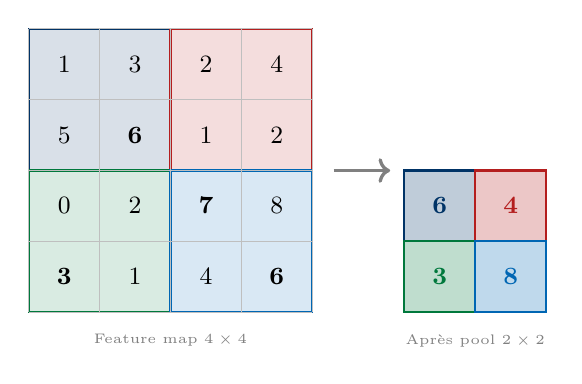
\begin{tikzpicture}[scale=0.90]
        % --- Input 4x4 hardcoded ---
        % Row 3 (top): 1 3 2 4
        % Row 2:       5 6 1 2
        % Row 1:       0 2 7 8
        % Row 0 (bot): 3 1 4 6

        % Zone bleue haut-gauche
        \draw[jedy_blue, thick, fill=jedy_blue!15] (0,2) rectangle (2,4);
        % Zone rouge haut-droite
        \draw[jedy_alert, thick, fill=jedy_alert!15] (2,2) rectangle (4,4);
        % Zone verte bas-gauche
        \draw[jedy_example, thick, fill=jedy_example!15] (0,0) rectangle (2,2);
        % Zone orange bas-droite
        \draw[jedy_mid, thick, fill=jedy_mid!15] (2,0) rectangle (4,2);

        % Grid lines
        \foreach \i in {0,...,4} {
          \draw[gray!50] (\i,0) -- (\i,4);
          \draw[gray!50] (0,\i) -- (4,\i);
        }

        % Values
        \node[font=\small] at (0.5,3.5) {1};
        \node[font=\small] at (1.5,3.5) {3};
        \node[font=\small] at (2.5,3.5) {2};
        \node[font=\small] at (3.5,3.5) {4};

        \node[font=\small] at (0.5,2.5) {5};
        \node[font=\small] at (1.5,2.5) {\textbf{6}};
        \node[font=\small] at (2.5,2.5) {1};
        \node[font=\small] at (3.5,2.5) {2};

        \node[font=\small] at (0.5,1.5) {0};
        \node[font=\small] at (1.5,1.5) {2};
        \node[font=\small] at (2.5,1.5) {\textbf{7}};
        \node[font=\small] at (3.5,1.5) {8};

        \node[font=\small] at (0.5,0.5) {\textbf{3}};
        \node[font=\small] at (1.5,0.5) {1};
        \node[font=\small] at (2.5,0.5) {4};
        \node[font=\small] at (3.5,0.5) {\textbf{6}};

        \node[font=\tiny, gray] at (2, -0.4) {Feature map $4 \times 4$};

        % Arrow
        \draw[->, very thick, gray] (4.3, 2) -- (5.1, 2);

        % Output 2x2
        \begin{scope}[xshift=5.3cm]
          \draw[jedy_blue, thick, fill=jedy_blue!25] (0,1) rectangle (1,2);
          \node[font=\small\bfseries, color=jedy_blue] at (0.5,1.5) {6};

          \draw[jedy_alert, thick, fill=jedy_alert!25] (1,1) rectangle (2,2);
          \node[font=\small\bfseries, color=jedy_alert] at (1.5,1.5) {4};

          \draw[jedy_example, thick, fill=jedy_example!25] (0,0) rectangle (1,1);
          \node[font=\small\bfseries, color=jedy_example] at (0.5,0.5) {3};

          \draw[jedy_mid, thick, fill=jedy_mid!25] (1,0) rectangle (2,1);
          \node[font=\small\bfseries, color=jedy_mid] at (1.5,0.5) {8};

          \node[font=\tiny, gray] at (1, -0.4) {Après pool $2 \times 2$};
        \end{scope}
      \end{tikzpicture}
    \end{column}
  \end{columns}
\end{frame}

% ============================================================
\section{Architecture CNN}
% ============================================================

\begin{frame}{Architecture Globale d'un CNN}
  \begin{columns}[T]
    \begin{column}{0.44\textwidth}
      \begin{block}{Partie 1 : Extraction de features}
        \begin{itemize}
          \item \textbf{Conv} + \textbf{ReLU} + \textbf{Pool} $\times N$
          \item Image $\to$ cartes de caractéristiques abstraites
          \item Taille spatiale $\downarrow$, profondeur (canaux) $\uparrow$
        \end{itemize}
      \end{block}
      \vspace{1pt}
      \begin{block}{Partie 2 : Classification}
        \begin{itemize}
          \item \textbf{Flatten} : cartes $\to$ vecteur 1D
          \item MLP classique (J2) pour la décision finale
          \item Sortie : logits $\to$ softmax $\to$ classes
        \end{itemize}
      \end{block}
      \begin{exampleblock}{\small MNIST : $[B,1,28,28] \to [B,10]$}
        \small 1 canal, $28\!\times\!28$ pixels, 10 classes
      \end{exampleblock}
    \end{column}
    \begin{column}{0.52\textwidth}
      \centering
      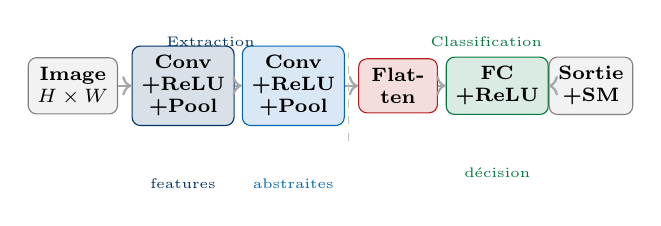
\begin{tikzpicture}[scale=0.70,
        blk/.style={rectangle, rounded corners=3pt, minimum height=0.65cm,
                    minimum width=1.0cm, align=center, font=\scriptsize\bfseries},
        arr/.style={->, thick, gray!70},
        lbl/.style={font=\tiny, text centered},
      ]
        \node[blk, draw=gray, fill=gray!10] (img) at (0,0)
          {Image\\$H\times W$};
        \node[blk, draw=jedy_blue, fill=jedy_blue!15] (c1) at (2.0,0)
          {Conv\\+ReLU\\+Pool};
        \node[blk, draw=jedy_mid, fill=jedy_mid!15] (c2) at (4.0,0)
          {Conv\\+ReLU\\+Pool};
        \node[blk, draw=jedy_alert, fill=jedy_alert!15] (fl) at (5.9,0)
          {Flat-\\ten};
        \node[blk, draw=jedy_example, fill=jedy_example!15] (fc) at (7.7,0)
          {FC\\+ReLU};
        \node[blk, draw=gray, fill=gray!10] (out) at (9.4,0)
          {Sortie\\+SM};

        \draw[arr] (img) -- (c1);
        \draw[arr] (c1)  -- (c2);
        \draw[arr] (c2)  -- (fl);
        \draw[arr] (fl)  -- (fc);
        \draw[arr] (fc)  -- (out);

        % Labels
        \node[lbl, color=jedy_blue, below=0.55cm of c1]  {features};
        \node[lbl, color=jedy_mid,  below=0.55cm of c2]  {abstraites};
        \node[lbl, color=jedy_example, below=0.55cm of fc] {décision};

        % Separator line between extraction and classification
        \draw[dashed, gray!50] (5.0, -1.0) -- (5.0, 0.6);
        \node[font=\tiny, color=jedy_blue]    at (2.5,  0.8) {Extraction};
        \node[font=\tiny, color=jedy_example] at (7.5,  0.8) {Classification};
      \end{tikzpicture}
    \end{column}
  \end{columns}
\end{frame}

% ============================================================
\section{Training Loop}
% ============================================================

\begin{frame}[fragile]{La Training Loop Standard}
  \begin{columns}[T]
    \begin{column}{0.37\textwidth}
      \begin{block}{Les 5 étapes rituelles}
        \begin{enumerate}\small
          \item \code{zero\_grad()} : efface les anciens gradients
          \item \code{model(x)} : forward pass
          \item \code{criterion(out, y)} : calcul de la perte
          \item \code{loss.backward()} : autograd
          \item \code{optimizer.step()} : mise à jour des poids
        \end{enumerate}
      \end{block}
      \smallskip
      \begin{alertblock}{\small Piège classique}
        \small Oublier \code{zero\_grad()} $\Rightarrow$ gradients \textbf{accumulés} $\Rightarrow$ divergence
      \end{alertblock}
    \end{column}
    \begin{column}{0.59\textwidth}
      \begin{lstlisting}[style=pythonstyle]
criterion = nn.CrossEntropyLoss()
optimizer = optim.Adam(model.parameters())

for epoch in range(n_epochs):
    for X, y in train_loader:
        # 1. Zero gradients
        optimizer.zero_grad()

        # 2. Forward pass
        output = model(X)

        # 3. Compute loss
        loss = criterion(output, y)

        # 4. Backward (autograd)
        loss.backward()

        # 5. Update weights
        optimizer.step()
      \end{lstlisting}
    \end{column}
  \end{columns}
\end{frame}

% ============================================================
\section{Récapitulatif}
% ============================================================

\begin{frame}{Récapitulatif : De J3-AM à la Vision}
  \begin{columns}[T]
    \begin{column}{0.48\textwidth}
      \begin{block}{Concepts maîtrisés}
        \begin{itemize}
          \item \textbf{Autograd} : graphe de calcul, chain rule, backward
          \item \textbf{Tenseurs} : généralisation vectorisée de \code{Value}
          \item \textbf{torch.nn} : couches, paramètres, forward
          \item \textbf{Convolutions} : localité, partage des poids
          \item \textbf{Pooling} : réduction, invariance
          \item \textbf{Training loop} : les 5 étapes rituelles
        \end{itemize}
      \end{block}
    \end{column}
    \begin{column}{0.48\textwidth}
      \begin{exampleblock}{Transition : MNIST $\to$ Vision complexe}
        \begin{itemize}
          \item MNIST ($28\times28$, 10 classes) : CNN simple
          \item ImageNet ($224\times224$, 1000 classes) : ResNet, VGG
          \item Détection d'objets : YOLO, Faster R-CNN
          \item Segmentation : U-Net
        \end{itemize}
      \end{exampleblock}
      \smallskip
      \begin{alertblock}{Demain : Séquences \& Attention}
        De la vision spatiale aux données \textbf{séquentielles}\\
        $\Rightarrow$ RNN, LSTM, Transformers
      \end{alertblock}
    \end{column}
  \end{columns}
\end{frame}

\end{document}
